% !TeX program = lualatex
% circuit-sim-lab-report — report4.tex
% Course 0714-EEE-2102, Circuit Simulation Laboratory
% Experiment 1 — transient and steady-state responses of RC circuits
%
% Compile (twice, from the project directory):
%   env lualatex -interaction=nonstopmode report4.tex

\documentclass[12pt,a4paper]{article}

% ----- Page geometry: A4, 1 inch margins all sides -----
\usepackage[a4paper,margin=1in]{geometry}

% ----- Times New Roman text with matching mathematical type -----
\usepackage{fontspec}
\setmainfont{Times New Roman}
\usepackage{unicode-math}
\setmathfont{TeX Gyre Termes Math}

% ----- Spacing: 1.5 line spacing, 6 pt paragraph spacing -----
\usepackage{setspace}
\onehalfspacing
\usepackage[skip=6pt]{parskip}

% ----- Math, SI units -----
\usepackage{amsmath}
\AtBeginDocument{%
	\setlength{\abovedisplayskip}{12pt}%
	\setlength{\belowdisplayskip}{12pt}%
	\setlength{\abovedisplayshortskip}{6pt}%
	\setlength{\belowdisplayshortskip}{12pt}}
\usepackage{siunitx}

% ----- Graphics, tables, captions, floats -----
\usepackage{graphicx}
\usepackage[american]{circuitikz}
\usepackage{tabularx}
\usepackage{xcolor}
\usepackage{colortbl}
\usepackage{caption}
\usepackage{float}
\graphicspath{{figures/}}

% ----- Lists: compact, guide-style itemization -----
\usepackage{enumitem}
\setlist{nosep, leftmargin=2em, label=\textbullet}

% ----- Front matter and PDF output -----
\usepackage{pdfpages}
\usepackage[hidelinks]{hyperref}

% ----- Ragged-right paragraph columns (Task 6 parameter table) -----
\usepackage{array}
\newcolumntype{P}[1]{>{\raggedright\arraybackslash}p{#1}}
\newcolumntype{Y}{>{\raggedright\arraybackslash}X}
\newcolumntype{Z}{>{\centering\arraybackslash}X}
\newcommand{\reporttablestyle}{%
	\small
	\renewcommand{\arraystretch}{1.25}%
	\setlength{\tabcolsep}{6pt}%
	\setlength{\arrayrulewidth}{0.4pt}%
	\arrayrulecolor{black!65}}


% ----- URL line breaking (reference [3]) -----
\usepackage{xurl}

% ----- Headings: bold, left-aligned, 16/14 pt -----
\usepackage{titlesec}
\titleformat{\section}
{\normalfont\fontsize{16}{20}\selectfont\bfseries\raggedright}{\thesection}{0.8em}{}
\titleformat{\subsection}
{\normalfont\fontsize{14}{18}\selectfont\bfseries\raggedright}{\thesubsection}{0.8em}{}
\titlespacing*{\section}{0pt}{*3}{*2}
\titlespacing*{\subsection}{0pt}{*2.5}{*1.5}
\titleformat{\paragraph}[block]
{\normalfont\fontsize{14}{18}\selectfont\bfseries\raggedright}{}{0pt}{}
\titlespacing*{\paragraph}{0pt}{12pt}{6pt}

\DeclareCaptionFont{ieeecaption}{\fontsize{12}{14}\selectfont}
\DeclareCaptionTextFormat{ieeetable}{\MakeUppercase{#1}}
\renewcommand{\thetable}{\Roman{table}}
\captionsetup{font={normalfont,ieeecaption}, labelfont=normalfont, textfont=normalfont}
\captionsetup[table]{name=TABLE, labelsep=newline, textformat=ieeetable,
	justification=centering, singlelinecheck=false, position=above, skip=6pt}
\captionsetup[figure]{name=Fig., labelsep=period, justification=justified,
	singlelinecheck=true, position=below, skip=6pt}

% ----- Page number: bottom-center -----
\usepackage{fancyhdr}
\pagestyle{fancy}
\fancyhf{}
\fancyfoot[C]{\thepage}
\renewcommand{\headrulewidth}{0pt}

% ----- Experiment number: sections then number N.1–N.10 -----
\newcommand{\expnumber}{1}
\renewcommand{\thesection}{\expnumber.\arabic{section}}

\begin{document}
	
	\begin{figure}[H]
		\centering
		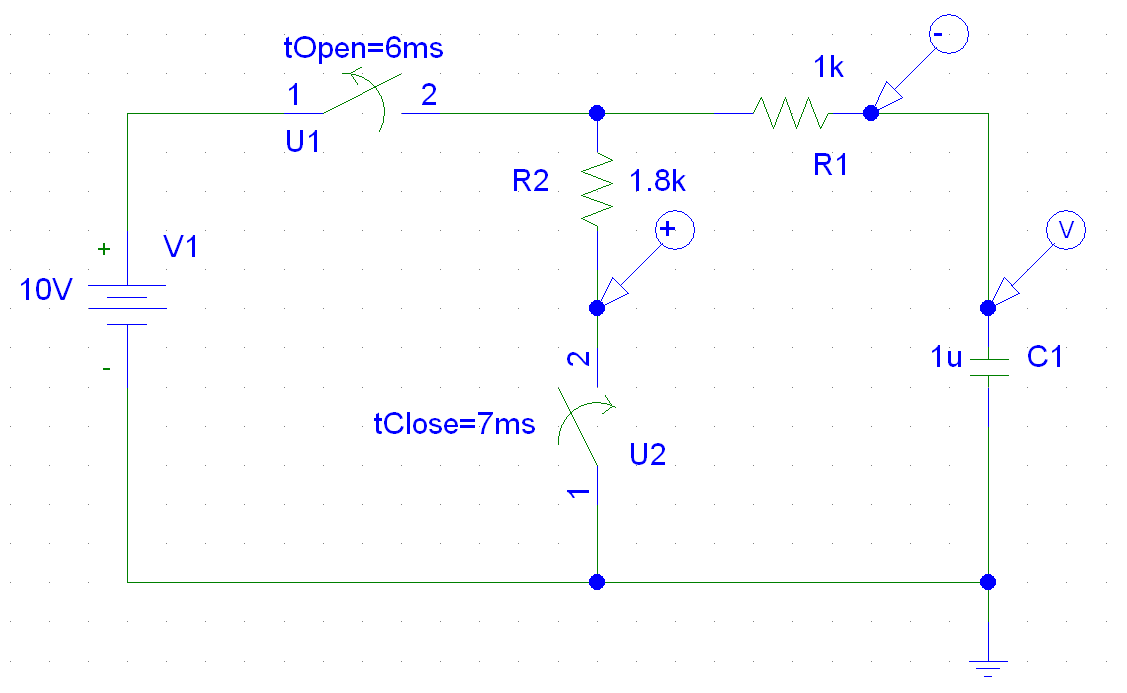
\includegraphics[width=0.85\textwidth,height=0.75\textheight,keepaspectratio]{circuit_task1,2.png}
		\caption{PSpice schematic of the switching RC circuit (Tasks 1 and 2): \SI{10}{\volt} DC source V1, \SI{1}{\kilo\ohm} charging
			resistor, \SI{1.8}{\kilo\ohm} discharge resistor, C1 =
			\SI{1}{\micro\farad}; U1 opens at $\symup{t}_{\mathit{open}} =
			\SI{6}{\milli\second}$ and U2 closes at $\symup{t}_{\mathit{close}} =
			\SI{7}{\milli\second}$.}
		\label{fig:schematic-switching}
	\end{figure}
	
	\begin{figure}[H]
		\centering
		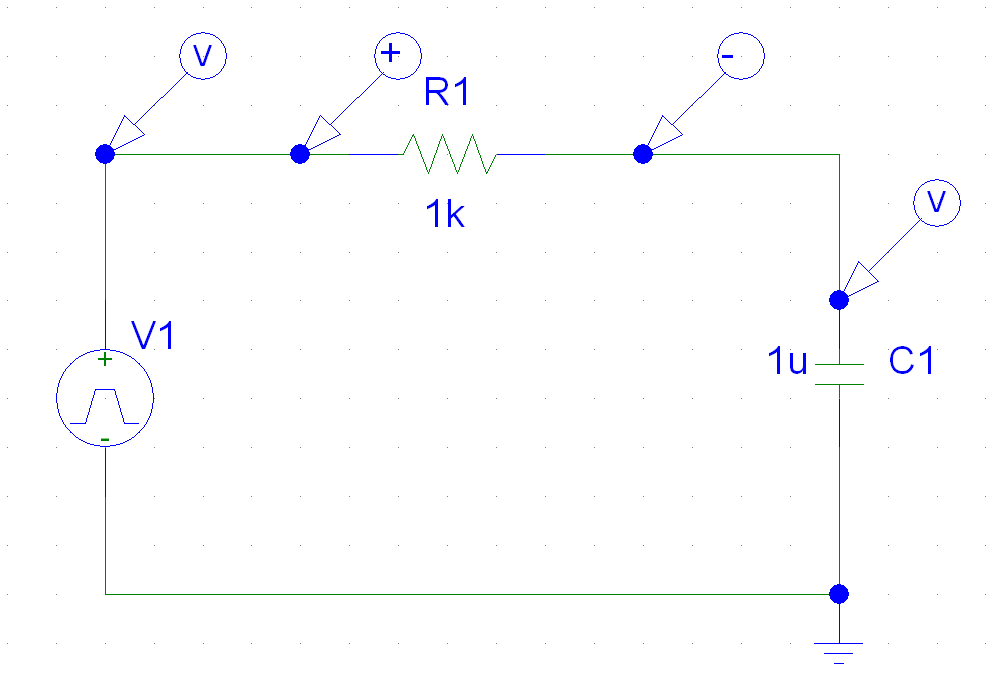
\includegraphics[width=0.8\textwidth,height=0.75\textheight,keepaspectratio]{circuit_task3.png}
		\caption{PSpice schematic of the pulse-driven RC circuit (Task 3):
			pulse source V1 (0--\SI{5}{\volt}, width \SI{5}{\milli\second},
			period \SI{10}{\milli\second}) in series with R1 =
			\SI{1}{\kilo\ohm} and C1 = \SI{1}{\micro\farad}.}
		\label{fig:schematic-pulse}
	\end{figure}
	
	\begin{figure}[H]
		\centering
		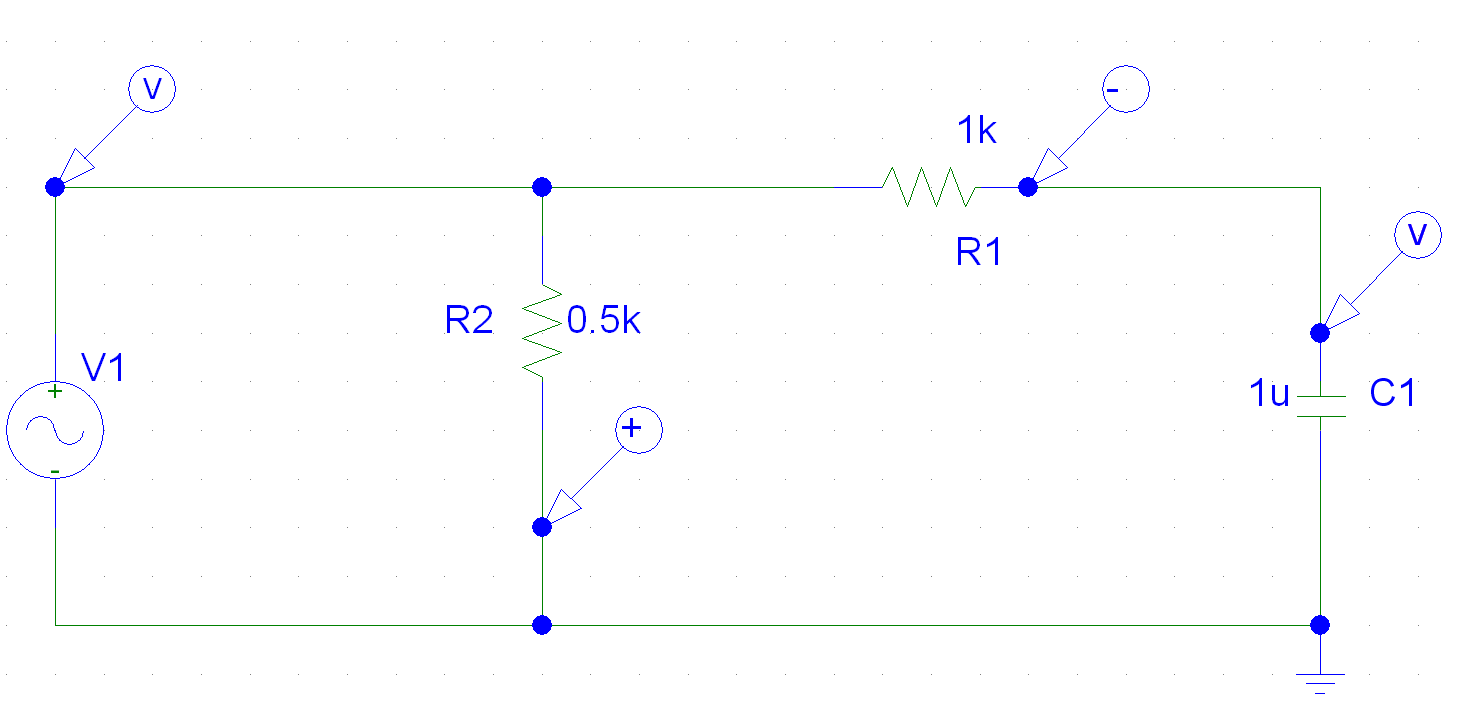
\includegraphics[width=0.85\textwidth,height=0.75\textheight,keepaspectratio]{circuit_task4,5.png}
		\caption{PSpice schematic of the sinusoidally driven RC circuit
			(Tasks 4 and 5): V1 = $10\sin(2\pi\cdot100 t -
			70^{\circ})$~V, \SI{500}{\ohm} shunt resistor across the source,
			\SI{1}{\kilo\ohm} series resistor, and C1 =
			\SI{1}{\micro\farad}; Task 5 adds the initial condition
			\texttt{IC = -8.2748}.}
		\label{fig:schematic-sine}
	\end{figure}
	
	\begin{figure}[H]
		\centering
		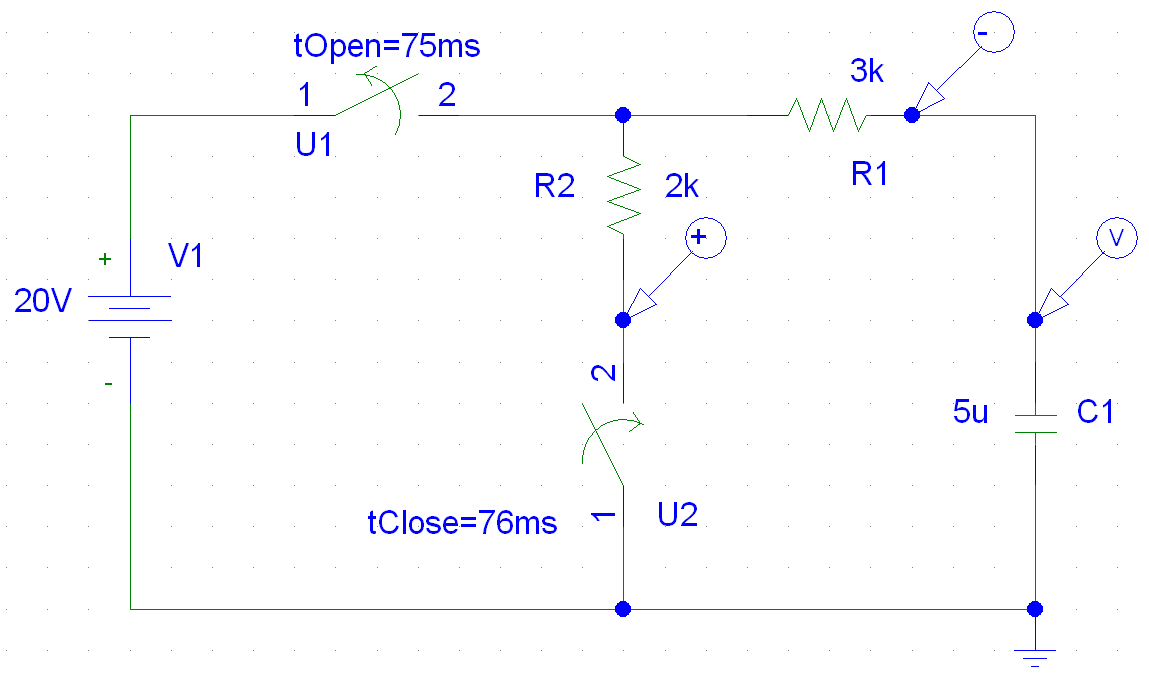
\includegraphics[width=0.85\textwidth,height=0.75\textheight,keepaspectratio]{circuit_task6a.png}
		\caption{PSpice schematic for Task 6a: \SI{20}{\volt} source,
			\SI{3}{\kilo\ohm} charging resistor, \SI{2}{\kilo\ohm}
			discharge resistor, and \SI{5}{\micro\farad} capacitor;
			U1 opens at \SI{75}{\milli\second} and U2 closes at
			\SI{76}{\milli\second}.}
		\label{fig:schematic-task6a}
	\end{figure}
	
	\begin{figure}[H]
		\centering
		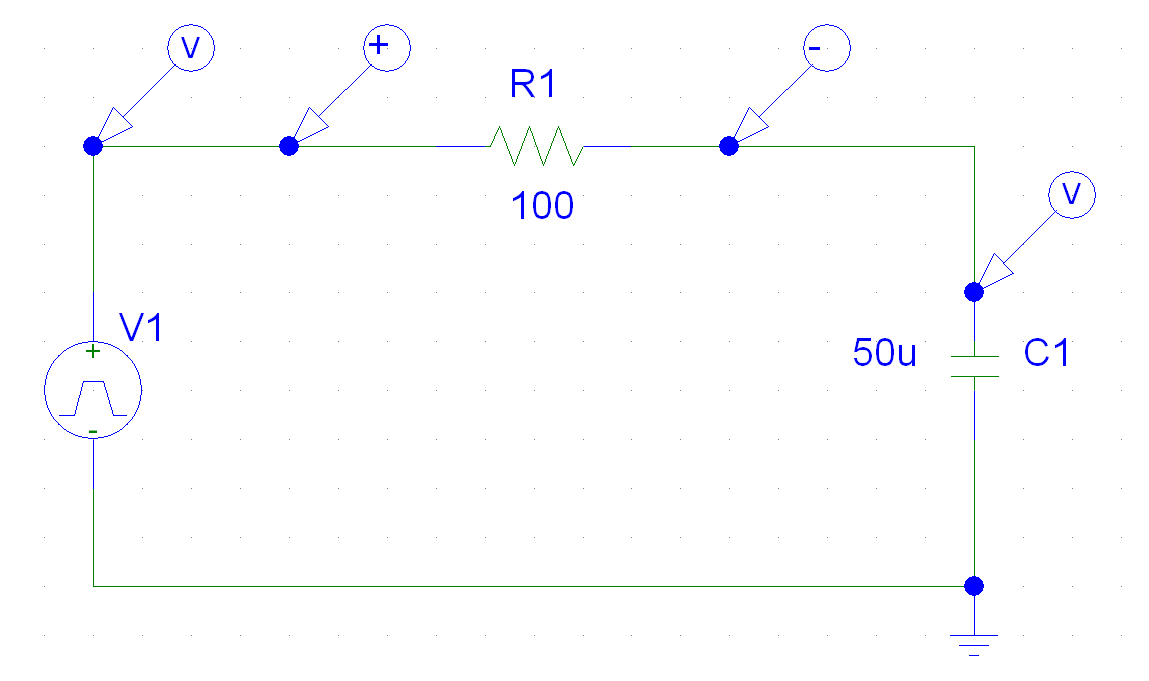
\includegraphics[width=0.8\textwidth,height=0.75\textheight,keepaspectratio]{circuit_task6b.png}
		\caption{PSpice schematic for Task 6b: pulse-driven RC circuit
			with R1 = \SI{100}{\ohm} and C1 = \SI{50}{\micro\farad}.}
		\label{fig:schematic-task6b}
	\end{figure}
	
	\begin{figure}[H]
		\centering
		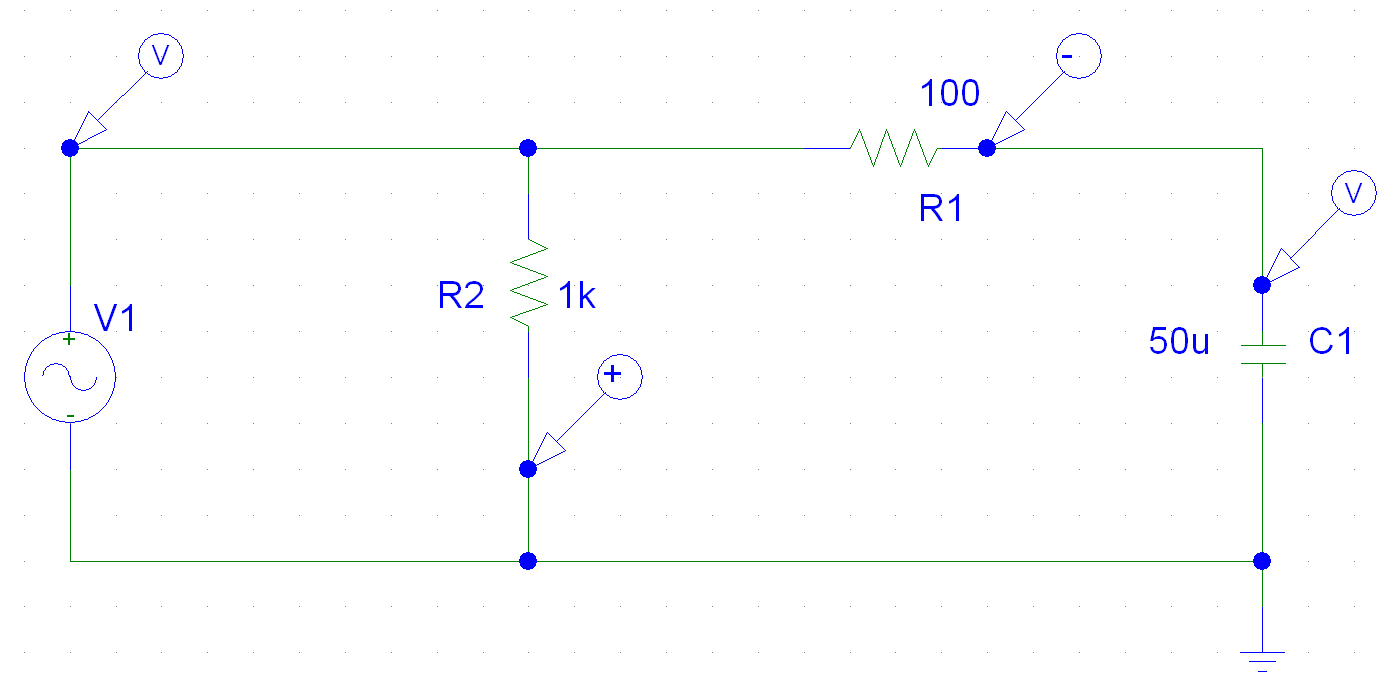
\includegraphics[width=0.85\textwidth,height=0.75\textheight,keepaspectratio]{circuit_task6c,d.png}
		\caption{PSpice schematic for Tasks 6c and 6d: sinusoidal source
			with a \SI{1}{\kilo\ohm} shunt resistor, \SI{100}{\ohm}
			series resistor, and \SI{50}{\micro\farad} capacitor;
			Task 6d applies the initial capacitor voltage
			\SI{-5.935}{\volt}.}
		\label{fig:schematic-task6cd}
	\end{figure}
	
	\begin{figure}[H]
		\centering
		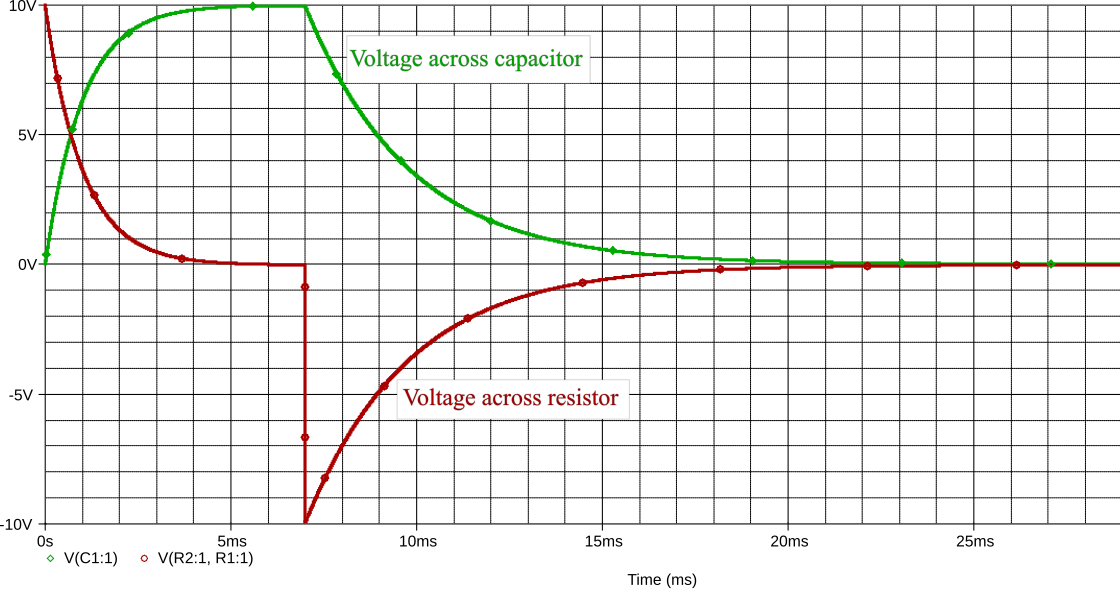
\includegraphics[width=\linewidth,height=0.4\textheight,keepaspectratio]{graph_task1,2.png}
		\caption{Simulated transient response of the switching RC circuit
			(Task 1): capacitor voltage charging during
			$0$--\SI{6}{\milli\second}, holding between
			\SI{6}{\milli\second} and \SI{7}{\milli\second}, and
			discharging after \SI{7}{\milli\second}.}
		\label{fig:task12}
	\end{figure}
	
	\begin{figure}[H]
		\centering
		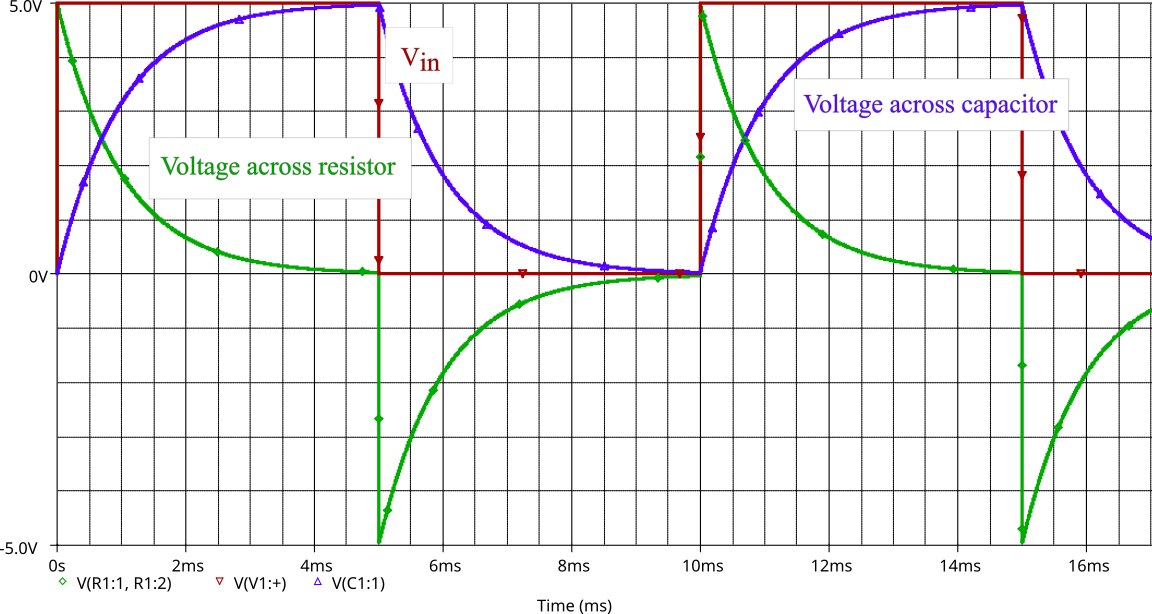
\includegraphics[width=\linewidth,height=0.4\textheight,keepaspectratio]{graph_task3.png}
		\caption{Simulated response of the RC circuit to the
			0--\SI{5}{\volt} pulse train (Task 3): the capacitor charges
			during each \SI{5}{\milli\second} on-interval and discharges
			during each \SI{5}{\milli\second} off-interval.}
		\label{fig:task3}
	\end{figure}
	
	\begin{figure}[H]
		\centering
		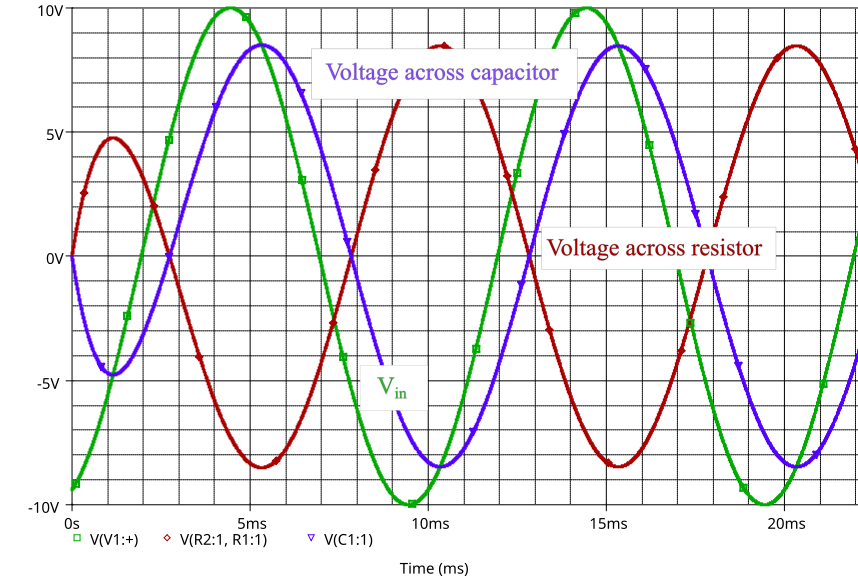
\includegraphics[width=\linewidth,height=0.4\textheight,keepaspectratio]{graph_task4.png}
		\caption{Simulated response of the RC circuit to
			$10\sin(2\pi\cdot100 t - 70^{\circ})$~\si{\volt} (Task 4): the capacitor
			voltage starts from zero and converges to the attenuated,
			phase-lagged steady-state sinusoid within about
			$5\tau = \SI{5}{\milli\second}$.}
		\label{fig:task4}
	\end{figure}
	
	\begin{figure}[H]
		\centering
		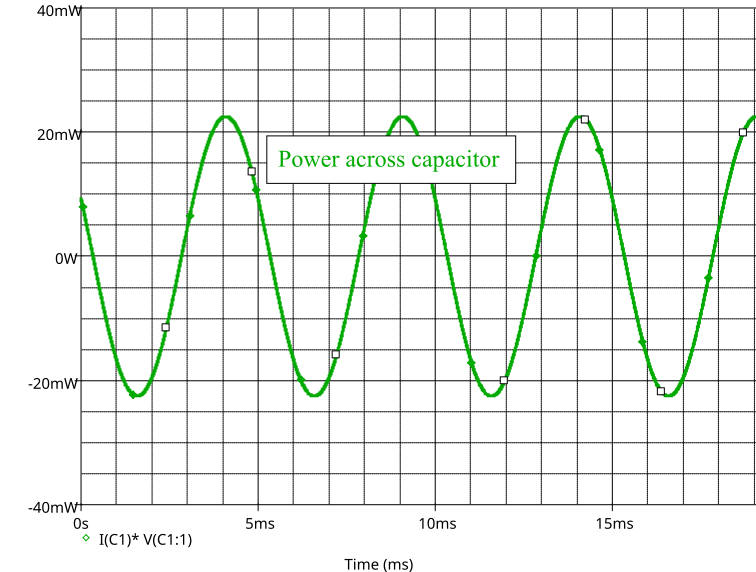
\includegraphics[width=\linewidth,height=0.4\textheight,keepaspectratio]{graph_task4_power.png}
		\caption{Instantaneous power of the capacitor for the Task 4 run:
			after the transient dies out the power oscillates symmetrically
			about zero with a peak of \SI{22.5}{\milli\watt}, indicating no
			net energy absorption in the steady state.}
		\label{fig:task4power}
	\end{figure}
	
	\begin{figure}[H]
		\centering
		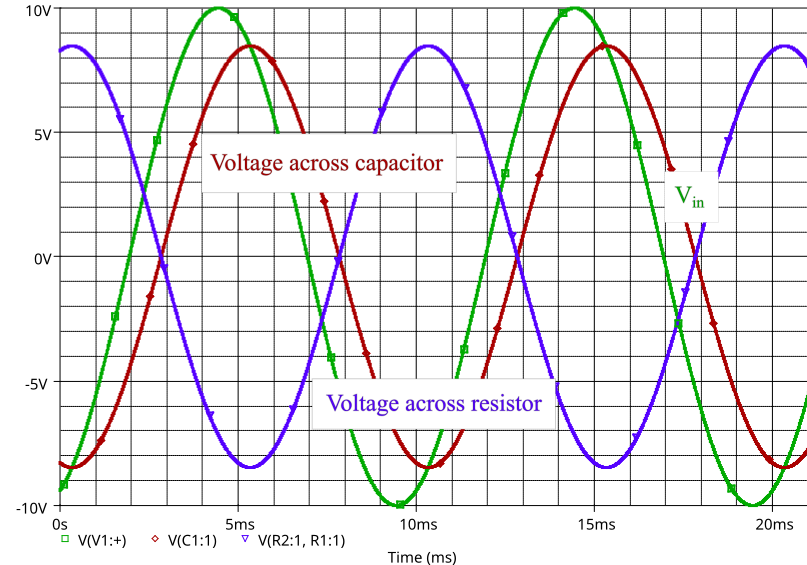
\includegraphics[width=\linewidth,height=0.4\textheight,keepaspectratio]{graph_task5.png}
		\caption{Task 5: with the initial condition
			\texttt{IC = -8.2748}, the capacitor voltage is a pure
			steady-state sinusoid from $t = 0$; no transient component is
			visible.}
		\label{fig:task5}
	\end{figure}
	
	\begin{figure}[H]
		\centering
		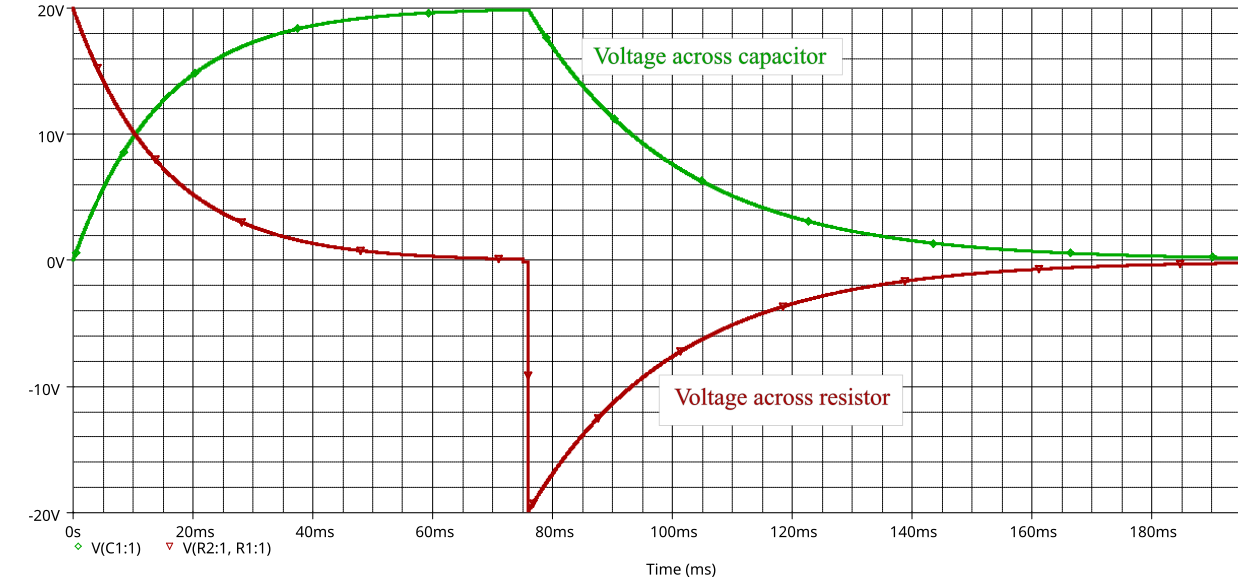
\includegraphics[width=\linewidth,height=0.4\textheight,keepaspectratio]{graph_task6a.png}
		\caption{Task 6a: response of the switching RC circuit with
			\SI{3}{\kilo\ohm} charging resistor, \SI{5}{\kilo\ohm} discharge
			path, $C = \SI{5}{\micro\farad}$, and \SI{20}{\volt} source:
			charging for \SI{75}{\milli\second} ($5\symup{\tau}_{\mathit{charge}}$), hold for
			\SI{1}{\milli\second}, discharging with
			$\symup{\tau}_{\mathit{discharge}} = \SI{25}{\milli\second}$.}
		\label{fig:task6a}
	\end{figure}
	
	\begin{figure}[H]
		\centering
		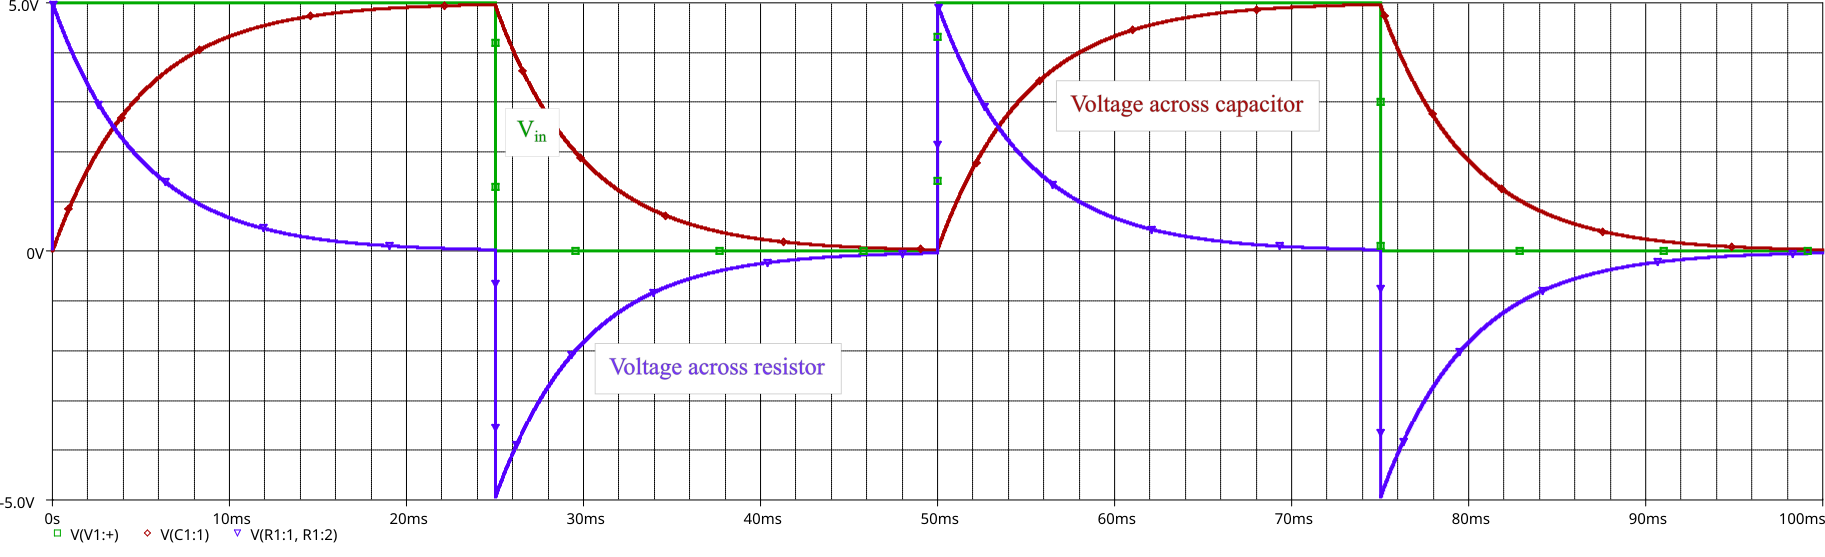
\includegraphics[width=\linewidth,height=0.4\textheight,keepaspectratio]{graph_task6b.png}
		\caption{Task 6b: response to the 0--\SI{5}{\volt} pulse train with
			$\tau = \SI{5}{\milli\second}$; each \SI{25}{\milli\second}
			half-cycle lasts $5\tau$, so the capacitor reaches
			$99.3\,\%$ of the pulse amplitude every cycle.}
		\label{fig:task6b}
	\end{figure}
	
		\begin{figure}[H]
		\centering
		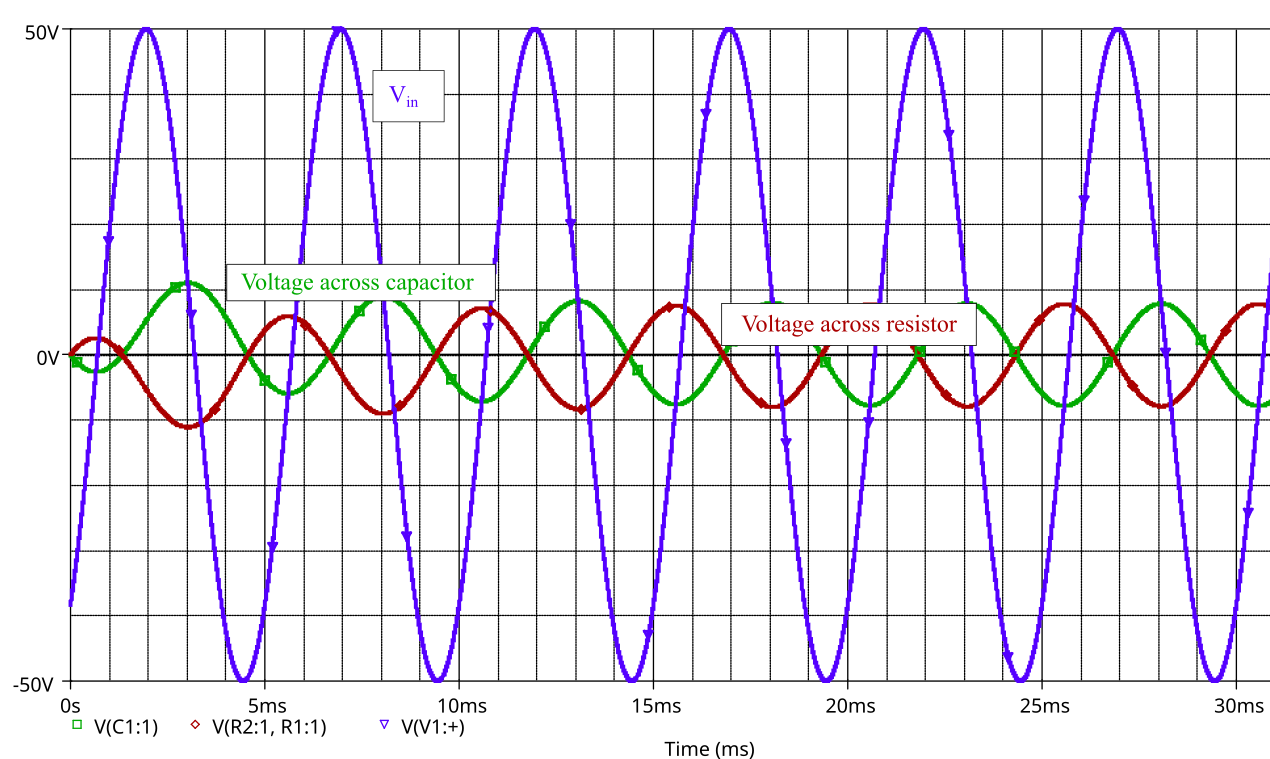
\includegraphics[width=\linewidth,height=0.4\textheight,keepaspectratio]{graph_task6c.png}
		\caption{Task 6c: response to
			$50\sin(2\pi\cdot200 t - 50^{\circ})$~\si{\volt} with $\tau =
			\SI{5}{\milli\second}$ ($\omega\tau = 2\pi$): the steady-state
			capacitor voltage is attenuated to \SI{7.86}{\volt} and lags the
			source by $81^\circ$; the \SI{5.935}{\volt} transient decays
			with $\tau = \SI{5}{\milli\second}$ and is still about
			\SI{15}{\milli\volt} at $t = \SI{30}{\milli\second}$.}
		\label{fig:task6c}
	\end{figure}
	

	\begin{figure}[H]
		\centering
		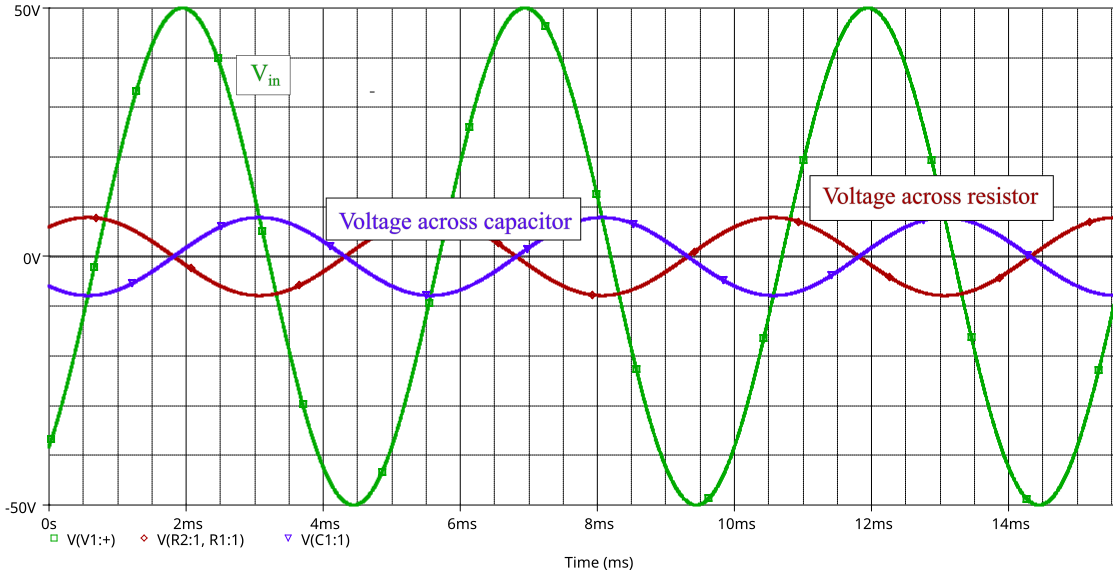
\includegraphics[width=\linewidth,height=0.4\textheight,keepaspectratio]{graph_task6d.png}
		\caption{Task 6d: with \texttt{.ic V(N002) = -5.935} the capacitor
			voltage is the pure steady-state sinusoid from $t = 0$; the
			transient of Fig.~\ref{fig:task6c} is absent.}
		\label{fig:task6d}
	\end{figure}

	\begin{figure}[H]
		\centering
		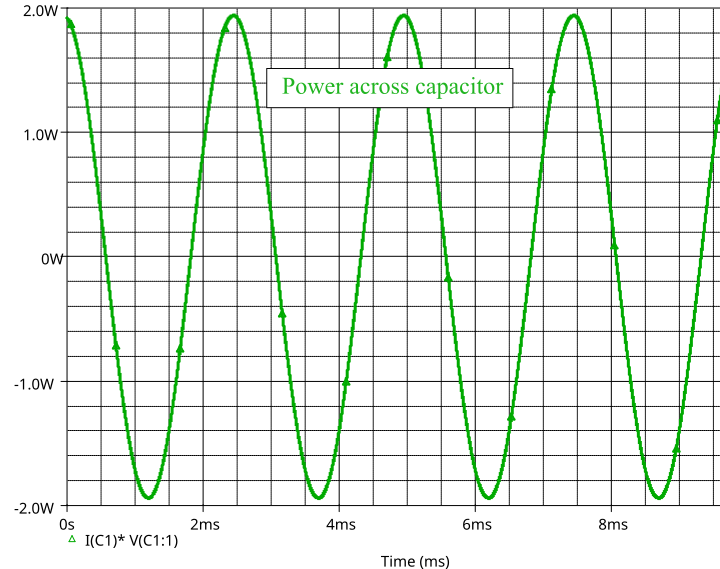
\includegraphics[width=\linewidth,height=0.4\textheight,keepaspectratio]{graph_task6d_power.png}
		\caption{Instantaneous capacitor power for Task 6d with the
			transient eliminated: the power alternates between positive
			and negative values as the capacitor stores and returns energy.}
		\label{fig:task6dpower}
	\end{figure}
	
	
\end{document}